% Teambook of AITU 1: Sorry, who are you?
% These codes should be guaranteed, fast enough, short and easy to type.

% twocolumn
% \documentclass[landscape, 8pt, a4paper, oneside, twocolumn]{extarticle}

\documentclass[landscape, 8pt, a4paper, oneside]{extreport}
\usepackage{kotex}
\usepackage{amssymb}
\usepackage{amsmath}
\usepackage{import}
\usepackage{enumitem}
\usepackage{multicol}
\usepackage{titlesec}
\usepackage{graphicx}

\usepackage{teamnote}

\teamnote{Astana IT University}{Sorry, who are you?}{Temirlan Baibolov, Arsen Muzhikov, Arman Issayev}{NERC 2024 (Astana, Kazakhstan)}

% smaller section title
% \titleformat{\subsection}{\normalfont\normalsize\bfseries}{\thesubsection}{1em}{}

\titlespacing*{\chapter}{0pt}{0pt}{0pt}
\titlespacing*{\section}{0pt}{0pt}{0pt}
\titlespacing*{\subsection}{0pt}{0pt}{0pt}

\ShowUsage
\ShowComplexity
\HideAuthor

\begin{document}

\maketitlepage
\pagebreak

\begin{multicols*}{3}

\setcounter{tocdepth}{0}
\tableofcontents

% break column
% \vfill\null\columnbreak

% Make Pagebreak if you want.
% \pagebreak

\chapter{Contest}

\Algorithm{template.cpp}
{}{}
{cpp}{code/contest/template.cpp}
{kactl}

\Algorithm{.bashrc}
{}{}
{sh}{code/contest/.bashrc}
{kactl}

\Algorithm{.vimrc}
{}{}
{text}{code/contest/.vimrc}
{kactl}

\Algorithm{hash.sh}
{}{}
{text}{code/contest/hash.sh}
{kactl}

\Algorithm{troubleshoot.txt}
{}{}
{text}{code/contest/troubleshoot.txt}
{kactl}

% Written by Anders Sjoqvist and Ulf Lundstrom, 2009
% The main sources are: tinyKACTL, Beta and Wikipedia

\chapter{Mathematics}

\section{Equations}
\[ax^2+bx+c=0 \Rightarrow x = \frac{-b\pm\sqrt{b^2-4ac}}{2a}\]

The extremum is given by $x = -b/2a$.

\[\begin{aligned}ax+by=e\\cx+dy=f\end{aligned}
\Rightarrow
\begin{aligned}x=\dfrac{ed-bf}{ad-bc}\\y=\dfrac{af-ec}{ad-bc}\end{aligned}\]

In general, given an equation $Ax = b$, the solution to a variable $x_i$ is given by
\[x_i = \frac{\det A_i'}{\det A} \]
where $A_i'$ is $A$ with the $i$'th column replaced by $b$.

\section{Recurrences}
If $a_n = c_1 a_{n-1} + \dots + c_k a_{n-k}$, and $r_1, \dots, r_k$ are distinct roots of $x^k - c_1 x^{k-1} - \dots - c_k$, there are $d_1, \dots, d_k$ s.t.
\[a_n = d_1r_1^n + \dots + d_kr_k^n. \]
Non-distinct roots $r$ become polynomial factors, e.g. $a_n = (d_1n + d_2)r^n$.

\section{Trigonometry}
\begin{align*}
\sin(v+w)&{}=\sin v\cos w+\cos v\sin w\\
\cos(v+w)&{}=\cos v\cos w-\sin v\sin w\\
\end{align*}
\begin{align*}
\tan(v+w)&{}=\dfrac{\tan v+\tan w}{1-\tan v\tan w}\\
\sin v+\sin w&{}=2\sin\dfrac{v+w}{2}\cos\dfrac{v-w}{2}\\
\cos v+\cos w&{}=2\cos\dfrac{v+w}{2}\cos\dfrac{v-w}{2}
\end{align*}
\[ (V+W)\tan(v-w)/2{}=(V-W)\tan(v+w)/2 \]
where $V, W$ are lengths of sides opposite angles $v, w$.
\begin{align*}
	a\cos x+b\sin x&=r\cos(x-\phi)\\
	a\sin x+b\cos x&=r\sin(x+\phi)
\end{align*}
where $r=\sqrt{a^2+b^2}, \phi=\operatorname{atan2}(b,a)$.

\section{Geometry}

\subsection{Triangles}
Side lengths: $a,b,c$\\
Semiperimeter: $p=\dfrac{a+b+c}{2}$\\
Area: $A=\sqrt{p(p-a)(p-b)(p-c)}$\\
Circumradius: $R=\dfrac{abc}{4A}$\\
Inradius: $r=\dfrac{A}{p}$\\
Length of median (divides triangle into two equal-area triangles): $m_a=\tfrac{1}{2}\sqrt{2b^2+2c^2-a^2}$\\
Length of bisector (divides angles in two): $s_a=\sqrt{bc\left[1-\left(\dfrac{a}{b+c}\right)^2\right]}$\\
Law of sines: $\dfrac{\sin\alpha}{a}=\dfrac{\sin\beta}{b}=\dfrac{\sin\gamma}{c}=\dfrac{1}{2R}$\\
Law of cosines: $a^2=b^2+c^2-2bc\cos\alpha$\\
Law of tangents: $\dfrac{a+b}{a-b}=\dfrac{\tan\dfrac{\alpha+\beta}{2}}{\tan\dfrac{\alpha-\beta}{2}}$\\

\subsection{Quadrilaterals}
With side lengths $a,b,c,d$, diagonals $e, f$, diagonals angle $\theta$, area $A$ and
magic flux $F=b^2+d^2-a^2-c^2$:

\[ 4A = 2ef \cdot \sin\theta = F\tan\theta = \sqrt{4e^2f^2-F^2} \]

 For cyclic quadrilaterals the sum of opposite angles is $180^\circ$,
$ef = ac + bd$, and $A = \sqrt{(p-a)(p-b)(p-c)(p-d)}$.

\subsection{Spherical coordinates}
\begin{center}
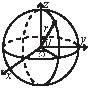
\includegraphics[width=25mm]{content/math/sphericalCoordinates}
\end{center}
\[\begin{array}{cc}
x = r\sin\theta\cos\phi & r = \sqrt{x^2+y^2+z^2}\\
y = r\sin\theta\sin\phi & \theta = \textrm{acos}(z/\sqrt{x^2+y^2+z^2})\\
z = r\cos\theta & \phi = \textrm{atan2}(y,x)
\end{array}\]

\section{Derivatives/Integrals}
\begin{align*}
	\dfrac{d}{dx}\arcsin x = \dfrac{1}{\sqrt{1-x^2}} &&& \dfrac{d}{dx}\arccos x = -\dfrac{1}{\sqrt{1-x^2}} \\
	\dfrac{d}{dx}\tan x = 1+\tan^2 x &&& \dfrac{d}{dx}\arctan x = \dfrac{1}{1+x^2} \\
	\int\tan ax = -\dfrac{\ln|\cos ax|}{a} &&& \int x\sin ax = \dfrac{\sin ax-ax \cos ax}{a^2} \\
	\int e^{-x^2} = \frac{\sqrt \pi}{2} \text{erf}(x) &&& \int xe^{ax}dx = \frac{e^{ax}}{a^2}(ax-1)
\end{align*}

Integration by parts:
\[\int_a^bf(x)g(x)dx = [F(x)g(x)]_a^b-\int_a^bF(x)g'(x)dx\]

\section{Sums}
\[ c^a + c^{a+1} + \dots + c^{b} = \frac{c^{b+1} - c^a}{c-1}, c \neq 1 \]
\begin{align*}
	1 + 2 + 3 + \dots + n &= \frac{n(n+1)}{2} \\
	1^2 + 2^2 + 3^2 + \dots + n^2 &= \frac{n(2n+1)(n+1)}{6} \\
	1^3 + 2^3 + 3^3 + \dots + n^3 &= \frac{n^2(n+1)^2}{4} \\
	1^4 + 2^4 + 3^4 + \dots + n^4 &= \frac{n(n+1)(2n+1)(3n^2 + 3n - 1)}{30} \\
\end{align*}

\section{Series}
$$e^x = 1+x+\frac{x^2}{2!}+\frac{x^3}{3!}+\dots,\,(-\infty<x<\infty)$$
$$\ln(1+x) = x-\frac{x^2}{2}+\frac{x^3}{3}-\frac{x^4}{4}+\dots,\,(-1<x\leq1)$$
$$\sqrt{1+x} = 1+\frac{x}{2}-\frac{x^2}{8}+\frac{2x^3}{32}-\frac{5x^4}{128}+\dots,\,(-1\leq x\leq1)$$
$$\sin x = x-\frac{x^3}{3!}+\frac{x^5}{5!}-\frac{x^7}{7!}+\dots,\,(-\infty<x<\infty)$$
$$\cos x = 1-\frac{x^2}{2!}+\frac{x^4}{4!}-\frac{x^6}{6!}+\dots,\,(-\infty<x<\infty)$$

\section{Probability theory}
Let $X$ be a discrete random variable with probability $p_X(x)$ of assuming the value $x$. It will then have an expected value (mean) $\mu=\mathbb{E}(X)=\sum_xxp_X(x)$ and variance $\sigma^2=V(X)=\mathbb{E}(X^2)-(\mathbb{E}(X))^2=\sum_x(x-\mathbb{E}(X))^2p_X(x)$ where $\sigma$ is the standard deviation. If $X$ is instead continuous it will have a probability density function $f_X(x)$ and the sums above will instead be integrals with $p_X(x)$ replaced by $f_X(x)$.

Expectation is linear:
\[\mathbb{E}(aX+bY) = a\mathbb{E}(X)+b\mathbb{E}(Y)\]
For independent $X$ and $Y$, \[V(aX+bY) = a^2V(X)+b^2V(Y).\]

\subsection{Discrete distributions}

\subsubsection{Binomial distribution}
The number of successes in $n$ independent yes/no experiments, each which yields success with probability $p$ is $\textrm{Bin}(n,p),\,n=1,2,\dots,\, 0\leq p\leq1$.
\[p(k)=\binom{n}{k}p^k(1-p)^{n-k}\]
\[\mu = np,\,\sigma^2=np(1-p)\]
$\textrm{Bin}(n,p)$ is approximately $\textrm{Po}(np)$ for small $p$.

\subsubsection{First success distribution}
The number of trials needed to get the first success in independent yes/no experiments, each which yields success with probability $p$ is $\textrm{Fs}(p),\,0\leq p\leq1$.
\[p(k)=p(1-p)^{k-1},\,k=1,2,\dots\]
\[\mu = \frac1p,\,\sigma^2=\frac{1-p}{p^2}\]

\subsubsection{Poisson distribution}
The number of events occurring in a fixed period of time $t$ if these events occur with a known average rate $\kappa$ and independently of the time since the last event is $\textrm{Po}(\lambda),\,\lambda=t\kappa$.
\[p(k)=e^{-\lambda}\frac{\lambda^k}{k!}, k=0,1,2,\dots\]
\[\mu=\lambda,\,\sigma^2=\lambda\]

\subsection{Continuous distributions}

\subsubsection{Uniform distribution}
If the probability density function is constant between $a$ and $b$ and 0 elsewhere it is $\textrm{U}(a,b),\,a<b$.
\[f(x) = \left\{
\begin{array}{cl}
\frac{1}{b-a} & a<x<b\\
0 & \textrm{otherwise}
\end{array}\right.\]
\[\mu=\frac{a+b}{2},\,\sigma^2=\frac{(b-a)^2}{12}\]

\subsubsection{Exponential distribution}
The time between events in a Poisson process is $\textrm{Exp}(\lambda),\,\lambda>0$.
\[f(x) = \left\{
\begin{array}{cl}
\lambda e^{-\lambda x} & x\geq0\\
0 & x<0
\end{array}\right.\]
\[\mu=\frac{1}{\lambda},\,\sigma^2=\frac{1}{\lambda^2}\]

\subsubsection{Normal distribution}
Most real random values with mean $\mu$ and variance $\sigma^2$ are well described by $\mathcal{N}(\mu,\sigma^2),\,\sigma>0$.
\[ f(x) = \frac{1}{\sqrt{2\pi\sigma^2}}e^{-\frac{(x-\mu)^2}{2\sigma^2}} \]
If $X_1 \sim \mathcal{N}(\mu_1,\sigma_1^2)$ and $X_2 \sim \mathcal{N}(\mu_2,\sigma_2^2)$ then
\[ aX_1 + bX_2 + c \sim \mathcal{N}(\mu_1+\mu_2+c,a^2\sigma_1^2+b^2\sigma_2^2) \]

\section{Markov chains}
A \emph{Markov chain} is a discrete random process with the property that the next state depends only on the current state.
Let $X_1,X_2,\ldots$ be a sequence of random variables generated by the Markov process.
Then there is a transition matrix $\mathbf{P} = (p_{ij})$, with $p_{ij} = \Pr(X_n = i | X_{n-1} = j)$,
and $\mathbf{p}^{(n)} = \mathbf P^n \mathbf p^{(0)}$ is the probability distribution for $X_n$ (i.e., $p^{(n)}_i = \Pr(X_n = i)$),
where $\mathbf{p}^{(0)}$ is the initial distribution.

% \subsubsection{Stationary distribution}
$\mathbf{\pi}$ is a stationary distribution if $\mathbf{\pi} = \mathbf{\pi P}$.
If the Markov chain is \emph{irreducible} (it is possible to get to any state from any state),
then $\pi_i = \frac{1}{\mathbb{E}(T_i)}$ where $\mathbb{E}(T_i)$  is the expected time between two visits in state $i$.
$\pi_j/\pi_i$ is the expected number of visits in state $j$ between two visits in state $i$.

For a connected, undirected and non-bipartite graph, where the transition probability is uniform among all neighbors, $\pi_i$ is proportional to node $i$'s degree.

% \subsubsection{Ergodicity}
A Markov chain is \emph{ergodic} if the asymptotic distribution is independent of the initial distribution.
A finite Markov chain is ergodic iff it is irreducible and \emph{aperiodic} (i.e., the gcd of cycle lengths is 1).
$\lim_{k\rightarrow\infty}\mathbf{P}^k = \mathbf{1}\pi$.

% \subsubsection{Absorption}
A Markov chain is an A-chain if the states can be partitioned into two sets $\mathbf{A}$ and $\mathbf{G}$, such that all states in $\mathbf{A}$ are absorbing ($p_{ii}=1$), and all states in $\mathbf{G}$ leads to an absorbing state in $\mathbf{A}$.
The probability for absorption in state $i\in\mathbf{A}$, when the initial state is $j$, is $a_{ij} = p_{ij}+\sum_{k\in\mathbf{G}} a_{ik}p_{kj}$.
The expected time until absorption, when the initial state is $i$, is $t_i = 1+\sum_{k\in\mathbf{G}}p_{ki}t_k$.


\chapter{Data structures}

\kactlimport{OrderStatisticTree.h}
\kactlimport{HashMap.h}
\kactlimport{SegmentTree.h}
\kactlimport{LazySegmentTree.h}
% \kactlimport{UnionFind.h}
\kactlimport{UnionFindRollback.h}
\kactlimport{SubMatrix.h}
\kactlimport{Matrix.h}
\kactlimport{LineContainer.h}
\kactlimport{Treap.h}
\kactlimport{FenwickTree.h}
\kactlimport{FenwickTree2d.h}
\kactlimport{RMQ.h}
\kactlimport{MoQueries.h}


\chapter{Numerical}

\section{Polynomials and recurrences}
    \Algorithm{Polynomial.h}
    {}{}
    {cpp}{code/numerical/Polynomial.h}
    {kactl}
    \Algorithm{PolyRoots.h}
    {}{}
    {cpp}{code/numerical/PolyRoots.h}
    {kactl}
    \Algorithm{PolyInterpolate.h}
    {}{}
    {cpp}{code/numerical/PolyInterpolate.h}
    {kactl}
    \Algorithm{BerlekampMassey.h}
    {}{}
    {cpp}{code/numerical/BerlekampMassey.h}
    {kactl}
    \Algorithm{LinearRecurrence.h}
    {}{}
    {cpp}{code/numerical/LinearRecurrence.h}
    {kactl}

\section{Optimization}
    \Algorithm{GoldenSectionSearch.h}
    {}{}
    {cpp}{code/numerical/GoldenSectionSearch.h}
    {kactl}
    \Algorithm{HillClimbing.h}
    {}{}
    {cpp}{code/numerical/HillClimbing.h}
    {kactl}
    \Algorithm{Integrate.h}
    {}{}
    {cpp}{code/numerical/Integrate.h}
    {kactl}
    \Algorithm{IntegrateAdaptive.h}
    {}{}
    {cpp}{code/numerical/IntegrateAdaptive.h}
    {kactl}
    \Algorithm{Simplex.h}
    {}{}
    {cpp}{code/numerical/Simplex.h}
    {kactl}

\section{Matrices}
    \Algorithm{Determinant.h}
    {}{}
    {cpp}{code/numerical/Determinant.h}
    {kactl}
    \Algorithm{IntDeterminant.h}
    {}{}
    {cpp}{code/numerical/IntDeterminant.h}
    {kactl}
    \Algorithm{SolveLinear.h}
    {}{}
    {cpp}{code/numerical/SolveLinear.h}
    {kactl}
    \Algorithm{SolveLinear2.h}
    {}{}
    {cpp}{code/numerical/SolveLinear2.h}
    {kactl}
    \Algorithm{SolveLinearBinary.h}
    {}{}
    {cpp}{code/numerical/SolveLinearBinary.h}
    {kactl}
    \Algorithm{MatrixInverse.h}
    {}{}
    {cpp}{code/numerical/MatrixInverse.h}
    {kactl}
    \Algorithm{Tridiagonal.h}
    {}{}
    {cpp}{code/numerical/Tridiagonal.h}
    {kactl}

\section{Fourier transforms}
    \Algorithm{FastFourierTransform.h}
    {}{}
    {cpp}{code/numerical/FastFourierTransform.h}
    {kactl}
    \Algorithm{FastFourierTransformMod.h}
    {}{}
    {cpp}{code/numerical/FastFourierTransformMod.h}
    {kactl}
    \Algorithm{NumberTheoreticTransform.h}
    {}{}
    {cpp}{code/numerical/NumberTheoreticTransform.h}
    {kactl}
    \Algorithm{FastSubsetTransform.h}
    {}{}
    {cpp}{code/numerical/FastSubsetTransform.h}
    {kactl}


\chapter{Number theory}

\section{Modular arithmetic}
    \Algorithm{ModularArithmetic.h}
    {}{}
    {cpp}{code/number-theory/ModularArithmetic.h}
    {kactl}
    \Algorithm{ModInverse.h}
    {}{}
    {cpp}{code/number-theory/ModInverse.h}
    {kactl}
    \Algorithm{ModPow.h}
    {}{}
    {cpp}{code/number-theory/ModPow.h}
    {kactl}
    \Algorithm{ModLog.h}
    {}{}
    {cpp}{code/number-theory/ModLog.h}
    {kactl}
    \Algorithm{ModSum.h}
    {}{}
    {cpp}{code/number-theory/ModSum.h}
    {kactl}
    \Algorithm{ModMulLL.h}
    {}{}
    {cpp}{code/number-theory/ModMulLL.h}
    {kactl}
    \Algorithm{ModSqrt.h}
    {}{}
    {cpp}{code/number-theory/ModSqrt.h}
    {kactl}

\section{Primality}
    \Algorithm{FastEratosthenes.h}
    {}{}
    {cpp}{code/number-theory/FastEratosthenes.h}
    {kactl}
    \Algorithm{MillerRabin.h}
    {}{}
    {cpp}{code/number-theory/MillerRabin.h}
    {kactl}
    \Algorithm{Factor.h}
    {}{}
    {cpp}{code/number-theory/Factor.h}
    {kactl}

\section{Divisibility}
    \Algorithm{euclid.h}
    {}{}
    {cpp}{code/number-theory/euclid.h}
    {kactl}
    \Algorithm{CRT.h}
    {}{}
    {cpp}{code/number-theory/CRT.h}
    {kactl}

	\subsection{Bézout's identity}
	For $a \neq $, $b \neq 0$, then $d=gcd(a,b)$ is the smallest positive integer for which there are integer solutions to
	$$ax+by=d$$
	If $(x,y)$ is one solution, then all solutions are given by
	$$\left(x+\frac{kb}{\gcd(a,b)}, y-\frac{ka}{\gcd(a,b)}\right), \quad k\in\mathbb{Z}$$

    \Algorithm{phiFunction.h}
    {}{}
    {cpp}{code/number-theory/phiFunction.h}
    {kactl}

\section{Fractions}
    \Algorithm{ContinuedFractions.h}
    {}{}
    {cpp}{code/number-theory/ContinuedFractions.h}
    {kactl}
    \Algorithm{FracBinarySearch.h}
    {}{}
    {cpp}{code/number-theory/FracBinarySearch.h}
    {kactl}

\section{Pythagorean Triples}
 The Pythagorean triples are uniquely generated by
 \[ a=k\cdot (m^{2}-n^{2}),\ \,b=k\cdot (2mn),\ \,c=k\cdot (m^{2}+n^{2}), \]
 with $m > n > 0$, $k > 0$, $m \bot n$, and either $m$ or $n$ even.

\section{Primes}
	$p=962592769$ is such that $2^{21} \mid p-1$, which may be useful. For hashing
	use 970592641 (31-bit number), 31443539979727 (45-bit), 3006703054056749
	(52-bit). There are 78498 primes less than 1\,000\,000.

	Primitive roots exist modulo any prime power $p^a$, except for $p = 2, a > 2$, and there are $\phi(\phi(p^a))$ many.
	For $p = 2, a > 2$, the group $\mathbb Z_{2^a}^\times$ is instead isomorphic to $\mathbb Z_2 \times \mathbb Z_{2^{a-2}}$.

\section{Estimates}
	$\sum_{d|n} d = O(n \log \log n)$.

	The number of divisors of $n$ is at most around 100 for $n < 5e4$, 500 for $n < 1e7$, 2000 for $n < 1e10$, 200\,000 for $n < 1e19$.

\section{Mobius Function}
\[
	\mu(n) = \begin{cases} 0 & n \textrm{ is not square free}\\ 1 & n \textrm{ has even number of prime factors}\\ -1 & n \textrm{ has odd number of prime factors}\\\end{cases}
\]
  Mobius Inversion:
  \[ g(n) = \sum_{d|n} f(d) \Leftrightarrow f(n) = \sum_{d|n} \mu(d)g(n/d) \]
  Other useful formulas/forms:

  $ \sum_{d | n} \mu(d) = [ n = 1] $ (very useful)

  $ g(n) = \sum_{n|d} f(d) \Leftrightarrow f(n) = \sum_{n|d} \mu(d/n)g(d)$

 $ g(n) = \sum_{1 \leq m \leq n} f(\left\lfloor\frac{n}{m}\right \rfloor ) \Leftrightarrow f(n) = \sum_{1\leq m\leq n} \mu(m)g(\left\lfloor\frac{n}{m}\right\rfloor)$


\chapter{Combinatorial}

\section{Permutations}
	\subsection{Factorial}
		\begin{center}
\begin{tabular}{l}
\begin{tabular}{c|c@{\ }c@{\ }c@{\ }c@{\ }c@{\ }c@{\ }c@{\ }c@{\ }c@{\ }c}
$n$  & 1 & 2 & 3 & 4  & 5   & 6   & 7    & 8     & 9      & 10\\
\hline
$n!$ & 1 & 2 & 6 & 24 & 120 & 720 & 5040 & 40320 & 362880 & 3628800\\
\end{tabular}\\
\begin{tabular}{c|c@{\ }c@{\ }c@{\ }c@{\ }c@{\ }c@{\ }c@{\ }c@{\ }c@{\ }c}
$n$  & 11    & 12    & 13    & 14     & 15     & 16     & 17\\
\hline
$n!$ & 4.0e7 & 4.8e8 & 6.2e9 & 8.7e10 & 1.3e12 & 2.1e13 & 3.6e14\\
\end{tabular}\\
\begin{tabular}{c|c@{\ }c@{\ }c@{\ }c@{\ }c@{\ }c@{\ }c@{\ }c@{\ }c@{\ }c}
$n$  & 20   & 25   & 30   & 40   & 50   & 100   & 150   & 171\\
\hline
$n!$ & 2e18 & 2e25 & 3e32 & 8e47 & 3e64 & 9e157 & 6e262 & \scriptsize{$>$DBL\_MAX}\\
\end{tabular}
\end{tabular}
\end{center}


        \Algorithm{IntPerm.h}
        {}{}
        {cpp}{code/combinatorial/IntPerm.h}
        {kactl}

	\subsection{Derangements}
		Permutations of a set such that none of the elements appear in their original position.
		\[ \mkern-2mu D(n) = (n-1)(D(n-1)+D(n-2)) = n D(n-1)+(-1)^n = \left\lfloor\frac{n!}{e}\right\rceil \]

	\subsection{Burnside's lemma}
		Given a group $G$ of symmetries and a set $X$, the number of elements of $X$ \emph{up to symmetry} equals
		 \[ {\frac {1}{|G|}}\sum _{{g\in G}}|X^{g}|, \]
		 where $X^{g}$ are the elements fixed by $g$ ($g.x = x$).

		 If $f(n)$ counts ``configurations'' (of some sort) of length $n$, we can ignore rotational symmetry using $G = \mathbb Z_n$ to get
		 \[ g(n) = \frac 1 n \sum_{k=0}^{n-1}{f(\text{gcd}(n, k))} = \frac 1 n \sum_{k|n}{f(k)\phi(n/k)}. \]

\section{Partitions and subsets}
	\subsection{Partition function}
		Number of ways of writing $n$ as a sum of positive integers, disregarding the order of the summands.
		\[ p(0) = 1,\ p(n) = \sum_{k \in \mathbb Z \setminus \{0\}}{(-1)^{k+1} p(n - k(3k-1) / 2)} \]
		\[ p(n) \sim 0.145 / n \cdot \exp(2.56 \sqrt{n}) \]

		\begin{center}
		\begin{tabular}{c|c@{\ }c@{\ }c@{\ }c@{\ }c@{\ }c@{\ }c@{\ }c@{\ }c@{\ }c@{\ }c@{\ }c@{\ }c}
			$n$    & 0 & 1 & 2 & 3 & 4 & 5 & 6  & 7  & 8  & 9  & 20  & 50  & 100 \\ \hline
			$p(n)$ & 1 & 1 & 2 & 3 & 5 & 7 & 11 & 15 & 22 & 30 & 627 & $\mathtt{\sim}$2e5 & $\mathtt{\sim}$2e8 \\
		\end{tabular}
		\end{center}

	\subsection{Lucas' Theorem}
		Let $n,m$ be non-negative integers and $p$ a prime. Write $n=n_kp^k+...+n_1p+n_0$ and $m=m_kp^k+...+m_1p+m_0$. Then $\binom{n}{m} \equiv \prod_{i=0}^k\binom{n_i}{m_i} \pmod{p}$.

    \Algorithm{Binomials}
    {}{}
    {cpp}{code/combinatorial/multinomial.h}
    {kactl}

\section{General purpose numbers}
	\subsection{Bernoulli numbers}
		EGF of Bernoulli numbers is $B(t)=\frac{t}{e^t-1}$ (FFT-able).
		$B[0,\ldots] = [1, -\frac{1}{2}, \frac{1}{6}, 0, -\frac{1}{30}, 0, \frac{1}{42}, \ldots]$

		Sums of powers:
		\small
		\[ \sum_{i=1}^n n^m = \frac{1}{m+1} \sum_{k=0}^m \binom{m+1}{k} B_k \cdot (n+1)^{m+1-k} \]
		\normalsize

		Euler-Maclaurin formula for infinite sums:
		\small
		\[ \sum_{i=m}^{\infty} f(i) = \int_m^\infty f(x) dx - \sum_{k=1}^\infty \frac{B_k}{k!}f^{(k-1)}(m) \]
		\[ \approx \int_{m}^\infty f(x)dx + \frac{f(m)}{2} - \frac{f'(m)}{12} + \frac{f'''(m)}{720} + O(f^{(5)}(m)) \]
		\normalsize

	\subsection{Stirling numbers of the first kind}
		Number of permutations on $n$ items with $k$ cycles.
		\begin{align*}
			&c(n,k) = c(n-1,k-1) + (n-1) c(n-1,k),\ c(0,0) = 1 \\
			&\textstyle \sum_{k=0}^n c(n,k)x^k = x(x+1) \dots (x+n-1)
		\end{align*}
		$c(8,k) = 8, 0, 5040, 13068, 13132, 6769, 1960, 322, 28, 1$ \\
		$c(n,2) = 0, 0, 1, 3, 11, 50, 274, 1764, 13068, 109584, \dots$

	\subsection{Eulerian numbers}
		Number of permutations $\pi \in S_n$ in which exactly $k$ elements are greater than the previous element. $k$ $j$:s s.t. $\pi(j)>\pi(j+1)$, $k+1$ $j$:s s.t. $\pi(j)\geq j$, $k$ $j$:s s.t. $\pi(j)>j$.
		$$E(n,k) = (n-k)E(n-1,k-1) + (k+1)E(n-1,k)$$
		$$E(n,0) = E(n,n-1) = 1$$
		$$E(n,k) = \sum_{j=0}^k(-1)^j\binom{n+1}{j}(k+1-j)^n$$

	\subsection{Stirling numbers of the second kind}
		Partitions of $n$ distinct elements into exactly $k$ groups.
		$$S(n,k) = S(n-1,k-1) + k S(n-1,k)$$
		$$S(n,1) = S(n,n) = 1$$
		$$S(n,k) = \frac{1}{k!}\sum_{j=0}^k (-1)^{k-j}\binom{k}{j}j^n$$

	\subsection{Bell numbers}
		Total number of partitions of $n$ distinct elements. $B(n) =$
		$1, 1, 2, 5, 15, 52, 203, 877, 4140, 21147, \dots$. For $p$ prime,
		\[ B(p^m+n)\equiv mB(n)+B(n+1) \pmod{p} \]

	\subsection{Labeled unrooted trees}
		\# on $n$ vertices: $n^{n-2}$ \\
		\# on $k$ existing trees of size $n_i$: $n_1n_2\cdots n_k n^{k-2}$ \\
		\# with degrees $d_i$: $(n-2)! / ((d_1-1)! \cdots (d_n-1)!)$

	\subsection{Catalan numbers}
		\[ C_n=\frac{1}{n+1}\binom{2n}{n}= \binom{2n}{n}-\binom{2n}{n+1} = \frac{(2n)!}{(n+1)!n!} \]
		\[ C_0=1,\ C_{n+1} = \frac{2(2n+1)}{n+2}C_n,\ C_{n+1}=\sum C_iC_{n-i} \]
		${C_n = 1, 1, 2, 5, 14, 42, 132, 429, 1430, 4862, 16796, 58786, \dots}$
		\begin{itemize}[noitemsep]
			\item sub-diagonal monotone paths in an $n\times n$ grid.
			\item strings with $n$ pairs of parenthesis, correctly nested.
			\item binary trees with with $n+1$ leaves (0 or 2 children).
			\item ordered trees with $n+1$ vertices.
			\item ways a convex polygon with $n+2$ sides can be cut into triangles by connecting vertices with straight lines.
			\item permutations of $[n]$ with no 3-term increasing subseq.
		\end{itemize}


\chapter{Graph}

\section{Network flow}
    \Algorithm{PushRelabel.h}
    {}{}
    {cpp}{code/graph/PushRelabel.h}
    {kactl}
    \Algorithm{MinCostMaxFlow.h}
    {}{}
    {cpp}{code/graph/MinCostMaxFlow.h}
    {kactl}
    \Algorithm{MinCut.h}
    {}{}
    {cpp}{code/graph/MinCut.h}
    {kactl}
    \Algorithm{GlobalMinCut.h}
    {}{}
    {cpp}{code/graph/GlobalMinCut.h}
    {kactl}
    \Algorithm{GomoryHu.h}
    {}{}
    {cpp}{code/graph/GomoryHu.h}
    {kactl}

\section{Matching}
    \Algorithm{hopcroftKarp.h}
    {}{}
    {cpp}{code/graph/hopcroftKarp.h}
    {kactl}
    \Algorithm{MinimumVertexCover.h}
    {}{}
    {cpp}{code/graph/MinimumVertexCover.h}
    {kactl}
    \Algorithm{WeightedMatching.h}
    {}{}
    {cpp}{code/graph/WeightedMatching.h}
    {kactl}
    \Algorithm{GeneralMatching.h}
    {}{}
    {cpp}{code/graph/GeneralMatching.h}
    {kactl}

\section{DFS algorithms}
    \Algorithm{BiconnectedComponents.h}
    {}{}
    {cpp}{code/graph/BiconnectedComponents.h}
    {kactl}
    \Algorithm{EulerWalk.h}
    {}{}
    {cpp}{code/graph/EulerWalk.h}
    {kactl}

\section{Coloring}
    \Algorithm{EdgeColoring.h}
    {}{}
    {cpp}{code/graph/EdgeColoring.h}
    {kactl}

\section{Heuristics}
    \Algorithm{MaximalCliques.h}
    {}{}
    {cpp}{code/graph/MaximalCliques.h}
    {kactl}
    \Algorithm{MaximumClique.h}
    {}{}
    {cpp}{code/graph/MaximumClique.h}
    {kactl}

\section{Trees}
    \Algorithm{CompressTree.h}
    {}{}
    {cpp}{code/graph/CompressTree.h}
    {kactl}
    \Algorithm{LinkCutTree.h}
    {}{}
    {cpp}{code/graph/LinkCutTree.h}
    {kactl}
    \Algorithm{DirectedMST.h}
    {}{}
    {cpp}{code/graph/DirectedMST.h}
    {kactl}

\section{Math}
	\subsection{Number of Spanning Trees}
		% I.e. matrix-tree theorem.
		% Test: stress-tests/graph/matrix-tree.cpp
		Create an $N\times N$ matrix \texttt{mat}, and for each edge $a \rightarrow b \in G$, do
		\texttt{mat[a][b]--, mat[b][b]++} (and \texttt{mat[b][a]--, mat[a][a]++} if $G$ is undirected).
		Remove the $i$th row and column and take the determinant; this yields the number of directed spanning trees rooted at $i$
		(if $G$ is undirected, remove any row/column).

	\subsection{Erdős–Gallai theorem}
		% Test: stress-tests/graph/erdos-gallai.cpp
		A simple graph with node degrees $d_1 \ge \dots \ge d_n$ exists iff $d_1 + \dots + d_n$ is even and for every $k = 1\dots n$,
		\[ \sum _{i=1}^{k}d_{i}\leq k(k-1)+\sum _{i=k+1}^{n}\min(d_{i},k). \]


\chapter{Geometry}

\section{Geometric primitives}
    \Algorithm{Point.h}
    {}{}
    {cpp}{code/geometry/Point.h}
    {kactl}
    \Algorithm{lineDistance.h}
    {}{}
    {cpp}{code/geometry/lineDistance.h}
    {kactl}
    \Algorithm{SegmentDistance.h}
    {}{}
    {cpp}{code/geometry/SegmentDistance.h}
    {kactl}
    \Algorithm{SegmentIntersection}
    {}{}
    {cpp}{code/geometry/SegmentIntersection.h}
    {kactl}
    \Algorithm{lineIntersection.h}
    {}{}
    {cpp}{code/geometry/lineIntersection.h}
    {kactl}
    \Algorithm{sideOf.h}
    {}{}
    {cpp}{code/geometry/sideOf.h}
    {kactl}
    \Algorithm{OnSegment.h}
    {}{}
    {cpp}{code/geometry/OnSegment.h}
    {kactl}
    \Algorithm{linearTransformation.h}
    {}{}
    {cpp}{code/geometry/linearTransformation.h}
    {kactl}
    \Algorithm{Angle.h}
    {}{}
    {cpp}{code/geometry/Angle.h}
    {kactl}

\section{Circles}
    \Algorithm{CircleIntersection.h}
    {}{}
    {cpp}{code/geometry/CircleIntersection.h}
    {kactl}
    \Algorithm{CircleTangents.h}
    {}{}
    {cpp}{code/geometry/CircleTangents.h}
    {kactl}
    \Algorithm{CirclePolygonIntersection.h}
    {}{}
    {cpp}{code/geometry/CirclePolygonIntersection.h}
    {kactl}
    \Algorithm{circumcircle}
    {}{}
    {cpp}{code/geometry/circumcircle.h}
    {kactl}
    \Algorithm{MinimumEnclosingCircle.h}
    {}{}
    {cpp}{code/geometry/MinimumEnclosingCircle.h}
    {kactl}

\section{Polygons}
    \Algorithm{InsidePolygon.h}
    {}{}
    {cpp}{code/geometry/InsidePolygon.h}
    {kactl}
    \Algorithm{PolygonArea.h}
    {}{}
    {cpp}{code/geometry/PolygonArea.h}
    {kactl}
    \Algorithm{PolygonCenter.h}
    {}{}
    {cpp}{code/geometry/PolygonCenter.h}
    {kactl}
    \Algorithm{PolygonCut}
    {}{}
    {cpp}{code/geometry/PolygonCut.h}
    {kactl}
    \Algorithm{ConvexHull.h}
    {}{}
    {cpp}{code/geometry/ConvexHull.h}
    {kactl}
    \Algorithm{HullDiameter.h}
    {}{}
    {cpp}{code/geometry/HullDiameter.h}
    {kactl}
    \Algorithm{PointInsideHull.h}
    {}{}
    {cpp}{code/geometry/PointInsideHull.h}
    {kactl}
    \Algorithm{LineHullIntersection.h}
    {}{}
    {cpp}{code/geometry/LineHullIntersection.h}
    {kactl}

\section{Misc. Point Set Problems}
    \Algorithm{ClosestPair.h}
    {}{}
    {cpp}{code/geometry/ClosestPair.h}
    {kactl}
    \Algorithm{kdTree.h}
    {}{}
    {cpp}{code/geometry/kdTree.h}
    {kactl}
    \Algorithm{FastDelaunay.h}
    {}{}
    {cpp}{code/geometry/FastDelaunay.h}
    {kactl}

\section{3D}
    \Algorithm{PolyhedronVolume.h}
    {}{}
    {cpp}{code/geometry/PolyhedronVolume.h}
    {kactl}
    \Algorithm{Point3D.h}
    {}{}
    {cpp}{code/geometry/Point3D.h}
    {kactl}
    \Algorithm{3dHull.h}
    {}{}
    {cpp}{code/geometry/3dHull.h}
    {kactl}
    \Algorithm{sphericalDistance.h}
    {}{}
    {cpp}{code/geometry/sphericalDistance.h}
    {kactl}


\chapter{Strings}

\Algorithm{Zfunc.h}
{}{}
{cpp}{code/strings/Zfunc.h}
{kactl}

\Algorithm{Manacher.h}
{}{}
{cpp}{code/strings/Manacher.h}
{kactl}

\Algorithm{MinRotation.h}
{}{}
{cpp}{code/strings/MinRotation.h}
{kactl}

\Algorithm{SuffixTree.h}
{}{}
{cpp}{code/strings/SuffixTree.h}
{kactl}

\Algorithm{AhoCorasick.h}
{}{}
{cpp}{code/strings/AhoCorasick.h}
{kactl}


\chapter{Various}

\section{Intervals}
    \Algorithm{IntervalContainer.h}
    {}{}
    {cpp}{code/various/IntervalContainer.h}
    {kactl}
    \Algorithm{IntervalCover.h}
    {}{}
    {cpp}{code/various/IntervalCover.h}
    {kactl}
    \Algorithm{ConstantIntervals.h}
    {}{}
    {cpp}{code/various/ConstantIntervals.h}
    {kactl}

\section{Misc. algorithms}
    \Algorithm{TernarySearch.h}
    {}{}
    {cpp}{code/various/TernarySearch.h}
    {kactl}
    \Algorithm{LIS.h}
    {}{}
    {cpp}{code/various/LIS.h}
    {kactl}
    \Algorithm{FastKnapsack.h}
    {}{}
    {cpp}{code/various/FastKnapsack.h}
    {kactl}

\section{Dynamic programming}
    \Algorithm{KnuthDP.h}
    {}{}
    {cpp}{code/various/KnuthDP.h}
    {kactl}
    \Algorithm{DivideAndConquerDP.h}
    {}{}
    {cpp}{code/various/DivideAndConquerDP.h}
    {kactl}

\section{Debugging tricks}
	\begin{itemize}
		\item \verb@signal(SIGSEGV, [](int) { _Exit(0); });@ converts segfaults into Wrong Answers.
			Similarly one can catch SIGABRT (assertion failures) and SIGFPE (zero divisions).
			\verb@_GLIBCXX_DEBUG@ failures generate SIGABRT (or SIGSEGV on gcc 5.4.0 apparently).
		\item \verb@feenableexcept(29);@ kills the program on NaNs (\texttt 1), 0-divs (\texttt 4), infinities (\texttt 8) and denormals (\texttt{16}).
	\end{itemize}

\section{Optimization tricks}
	\verb@__builtin_ia32_ldmxcsr(40896);@ disables denormals (which make floats 20x slower near their minimum value).
	\subsection{Bit hacks}
		\begin{itemize}
			\item \verb@x & -x@ is the least bit in \texttt{x}.
			\item \verb@for (int x = m; x; ) { --x &= m; ... }@ loops over all subset masks of \texttt{m} (except \texttt{m} itself).
			\item \verb@c = x&-x, r = x+c; (((r^x) >> 2)/c) | r@ is the next number after \texttt{x} with the same number of bits set.
			\item \verb@rep(b,0,K) rep(i,0,(1 << K))@ \\ \verb@  if (i & 1 << b) D[i] += D[i^(1 << b)];@ computes all sums of subsets.
		\end{itemize}
	\subsection{Pragmas}
		\begin{itemize}
			\item \lstinline{#pragma GCC optimize ("Ofast")} will make GCC auto-vectorize loops and optimizes floating points better.
			\item \lstinline{#pragma GCC target ("avx2")} can double performance of vectorized code, but causes crashes on old machines.
			\item \lstinline{#pragma GCC optimize ("trapv")} kills the program on integer overflows (but is really slow).
		\end{itemize}
    \Algorithm{FastMod.h}
    {}{}
    {cpp}{code/various/FastMod.h}
    {kactl}
    \Algorithm{FastInput.h}
    {}{}
    {cpp}{code/various/FastInput.h}
    {kactl}
    \Algorithm{BumpAllocator.h}
    {}{}
    {cpp}{code/various/BumpAllocator.h}
    {kactl}
    \Algorithm{SmallPtr.h}
    {}{}
    {cpp}{code/various/SmallPtr.h}
    {kactl}
    \Algorithm{BumpAllocatorSTL.h}
    {}{}
    {cpp}{code/various/BumpAllocatorSTL.h}
    {kactl}
    \Algorithm{SIMD.h}
    {}{}
    {cpp}{code/various/SIMD.h}
    {kactl}


\end{multicols*}

\end{document}